\documentclass[11pt, reqno, letterpaper, twoside]{amsart}
\linespread{1.2}
\usepackage[margin=1.25in]{geometry}

\usepackage{amssymb, bm, mathtools}
\usepackage[usenames,dvipsnames,svgnames,table]{xcolor}
\usepackage[pdftex, xetex]{graphicx}
\usepackage{enumerate, setspace}
\usepackage{float, colortbl, tabularx, longtable, multirow, subcaption, environ, wrapfig, textcomp, booktabs}
\usepackage{appendix}
\usepackage{pgf, tikz, framed}
\usepackage[normalem]{ulem}
\usetikzlibrary{arrows,positioning,automata,shadows,fit,shapes}
\usepackage[english]{babel}
\usepackage{todonotes}
\usepackage{hyperref}
\usepackage{hhline}
\usepackage{microtype}
\usepackage[numbers]{natbib}
\microtypecontext{spacing=nonfrench}

\usepackage{times}
\title{DevDAgger: Data Efficient Visual Imitation Learning}
\author{ Kun Huang [huangkun@seas.upenn.edu]\\
Zhihao Ruan [ruanzh@seas.upenn.edu] \\
}

\begin{document}
% \begin{center} \Large \bfseries DevDAgger: Data Efficient Visual Imitation
%     Learning Through CNN and Gaussian Processes \end{center}

\begin{abstract}
	DAgger is a well-known online imitation learning algorithm in robot planning
	and control problems. Traditional DAggers suffer from the problem of high
	expert querying rate and could be costly under situations where expert
	querying is expensive. Moreover, traditional DAgger has not yet developed a
	state-of-the-art solution for vision-based planning and control. We propose
	DevDAgger, a vision-based data-efficient DAgger algorithm based on CNN and
	Gaussian Processes (GP) targeting low expert querying rate and visual
	imitation learning. We demonstrated our algorithm on the simple cart-pole
	problem and showed that state-based DevDAgger outperforms Vanilla DAgger in
	both performance and expert querying rate.
\end{abstract}

\maketitle

\section{Introduction}
Imitation learning is commonly used in planning and control in high-dimensional
state space with non-linear dynamical model in robotics. It offers robots the
ability to manipulate in complex environment without explicitly modelling the
environment by imitating the control actions from an expert (i.e., human).
Dataset Aggregation (DAgger) \cite{dagger}, in particular, is a popular online
imitation learning algorithm that trains the controller while aggregating new
data queried from the expert simultaneously. Traditional DAgger uses a neural
network to train the controller, requiring lots of expert data which is often
costly to obtain in many situations. This can actually be improved by replacing
the neural network with Gaussian Process (GP), which is a commonly used
model-free data efficient technique for regression tasks. Recent literature also
shows a particular interest in vision-based robotic planning and control
problems (visuomotor control) \cite{vision-based-RL,ebert2018visual,xie2018few}.
As a consequence, we propose a \emph{Data-Efficient Vision-based DAgger
	(DevDAgger)} algorithm for imitation learning tasks, combining the advantage of
Gaussian Process and latent representation learning with Convolutional Neural
Networks (CNNs).

\section{Related Work}
Imitation learning, as a supervised learning algorithm for robotic planning and
control, has long been a significant part in robotic research. A great variety
of approaches has been proposed for the traditional imitation learning tasks. On
one hand, many approaches has attempted to incorporate \textit{parametric
	models} to the imitation learning problem, such as dynamic movement primitives
(DMP) \cite{dmp}, Gaussian mixture models (GMM) \cite{gmm-for-IL}, and
probabilistic movement primitives (ProMP) \cite{ProMP}. On the other hand,
recent literature has also shown an extensive attention to
\textit{non-parametric models}, such as kernelized movement primitives (KMP)
\cite{non-parametric-il} and linearly constrained kernelized movement primitives
(LC-KMP) \cite{non-parametric-il-linear-constraints}.

DAgger, as an online imitation learning algorithm, was proposed in 2011 by
constantly aggregating data from the expert and imitating expert's behaviors
\cite{dagger}. Recent works have addressed some drawbacks of DAgger by improving
the expert data querying efficiency \cite{safe-dagger}. Uncertainty estimation
was also introduced to DAgger by EnsembleDAgger \cite{ensemble-dagger} to
improve the training-time safety.

Gaussian Processes (GP) itself has been a simple yet powerful non-parametric
model for general regression tasks. Traditional exact GP suffers from the
limitation of dataset in order to achieve reasonable amount of training time and
thus cannot be put into direct use in large scale learning tasks. However, the
computational efficiency of exact GP has recently been greatly improved by
GPyTorch \cite{exact-gp-million,GPyTorch}. By leveraging the power of GPyTorch,
exact GP has now become a new option for \textit{non-parametric} imitation
learning. EnsembleDAgger also attempts to incorporate ensembles and Monte-Carlo
methods as an approximation to exact GP \cite{ensemble-dagger}.

To summarize, we decided to utilize the power of exact GP in our DAgger
solution. We also incorporated the use of CNN to achieve vision-based planning
and control as an extra layer to the traditional DAgger pipeline. Meanwhile,
although GP suffers from the curse of dimensionality, recent works have shown
that mapping the structured high-dimensional inputs to latent space
\cite{grosnit2021high} dramatically expands the capability of GP.

\section{Approach}
Our proposed DevDAgger aims to provide a fast and data-efficient framework for
vision-based online imitation learning, or DAgger. As discussed above, the
existing variants of DAgger still attempts to use various approximations to GP
for uncertainty estimation, and has not yet incorporated vision-based planning
and control. Therefore, our proposed DevDAgger is composed of two parts: a novel
GP-based probabilistic visuomotor controller and an uncertainty-based decision
rule for DAgger to optimize expert query frequency.

\subsection{Problem Formulation}
In the context of general imitation learning, one would need the following
definitions: a \textit{novice} policy, an \textit{expert} policy, a well-defined
state space and a well-defined action space. Imitation learning generally trains
the novice to produce action $a_t$ exactly as the expert given some current
observation of the state $o_t$.

DAgger works as an online algorithm for imitation learning. Figure
\ref{fig:dagger_diagram} illustrates the workflow of a general DAgger. DAgger
collects dataset and trains the novice as the novice acts out in the
environment. Given some observations $o_t$ from the environment, both novice and
expert would generate their own actions $a_\text{nov}$ and $a_\text{exp}$. A
pre-defined decision rule would then choose an action $a_t$ and append the
observation-action pair $(o_t,a_t)$ to the dataset. The novice then gets trained
and observes a new $o_t$ in the next iteration.

As more and more iteration takes place, the novice gets trained for more and
more times and would act more and more similar to the expert. The decision rule
decides whether the novice action $a_\text{nov}$ or the expert action
$a_\text{exp}$ should be added to the dataset for the next training. There
should always be some novice actions in the dataset to ensure that the novice
policy is generalizable to unvisited states.
\begin{figure}[htbp!]
	\centering
	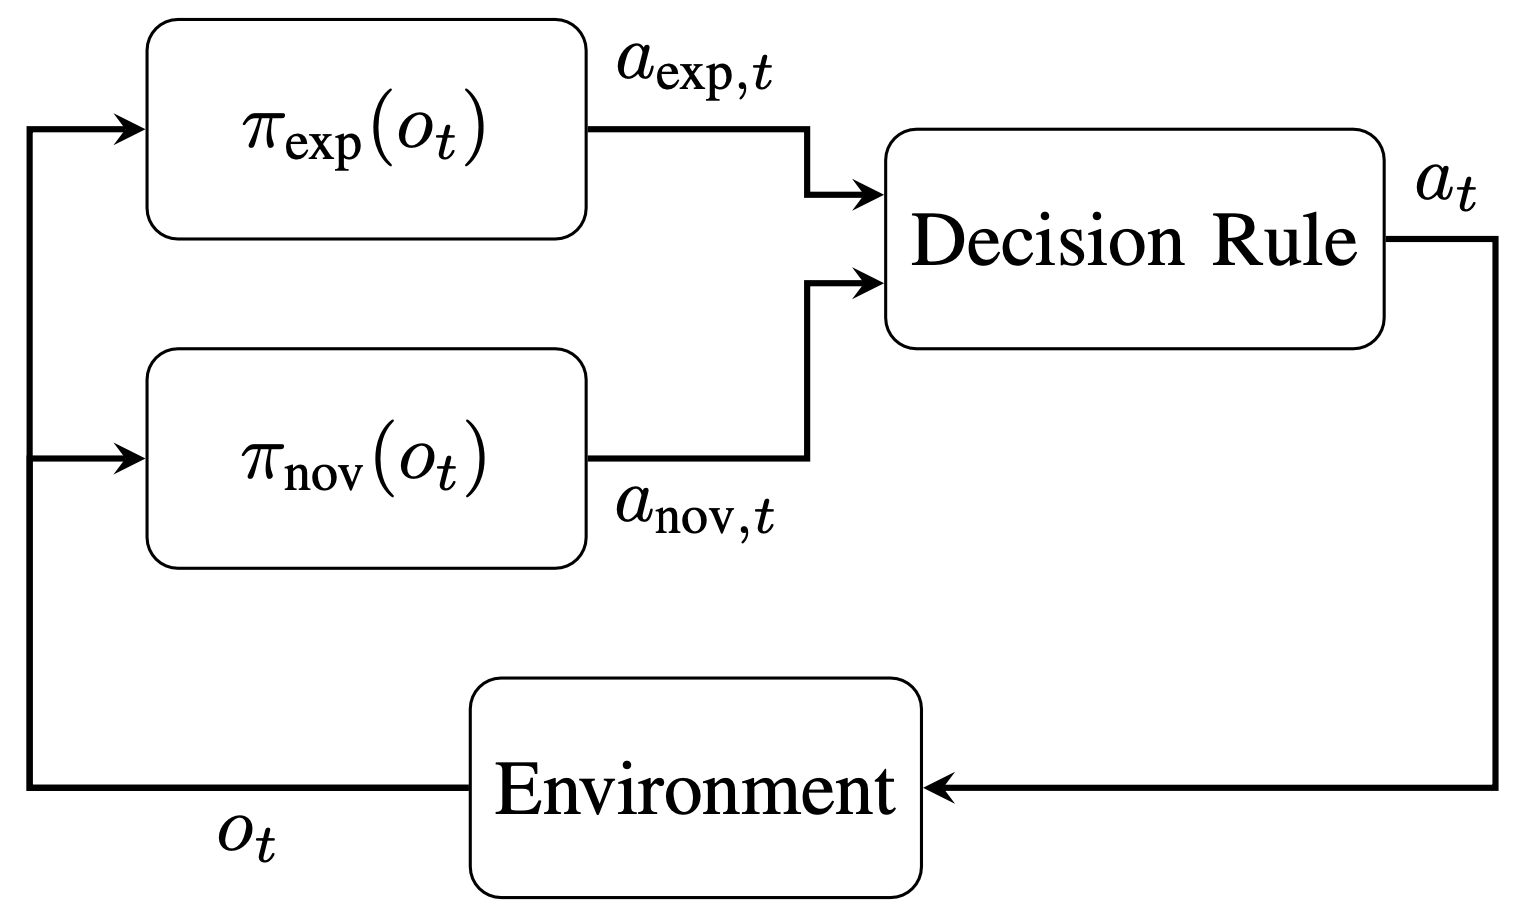
\includegraphics[width=0.5\linewidth]{imgs/dagger_diagram.png}
	\caption{Illustration of workflow of general DAgger \cite{ensemble-dagger}.}
	\label{fig:dagger_diagram}
\end{figure}

\subsection{Imitation Learning with Gaussian Processes}
Our algorithm starts with an observation-action pair $(o_t, a_t)$ from the
dataset. We first map the visual inputs $o_t$ into some latent space using the
CNN defined in Figure \ref{fig:conv_diagram}. Given the colored visual inputs,
we resize the images to be $3\times 64\times 64$ and stack the visual inputs
from 2 consecutive frames together in the color dimension in order to provide
speed information to the CNN, forming a final input of size $6\times 64\times
	64$. The images are then forwarded through the CNN and produces the
corresponding latent space feature points $z_t$. All convolutional layers use
the SAME padding. Although Figure \ref{fig:conv_diagram} only shows 2 sets of
convolution layers, there can be multiple sets of convolution layers in the CNN
architecture and this is a hyperparameter that should be tuned according to
different environments and robot dynamics models.

The output dimension of the linear layers of the CNN are shrunk by a factor of 4
in each layer. The linear layers would finally produce a latent space feature
point $z_t$ according to each $o_t$.

\begin{figure}[htbp!]
	\centering
	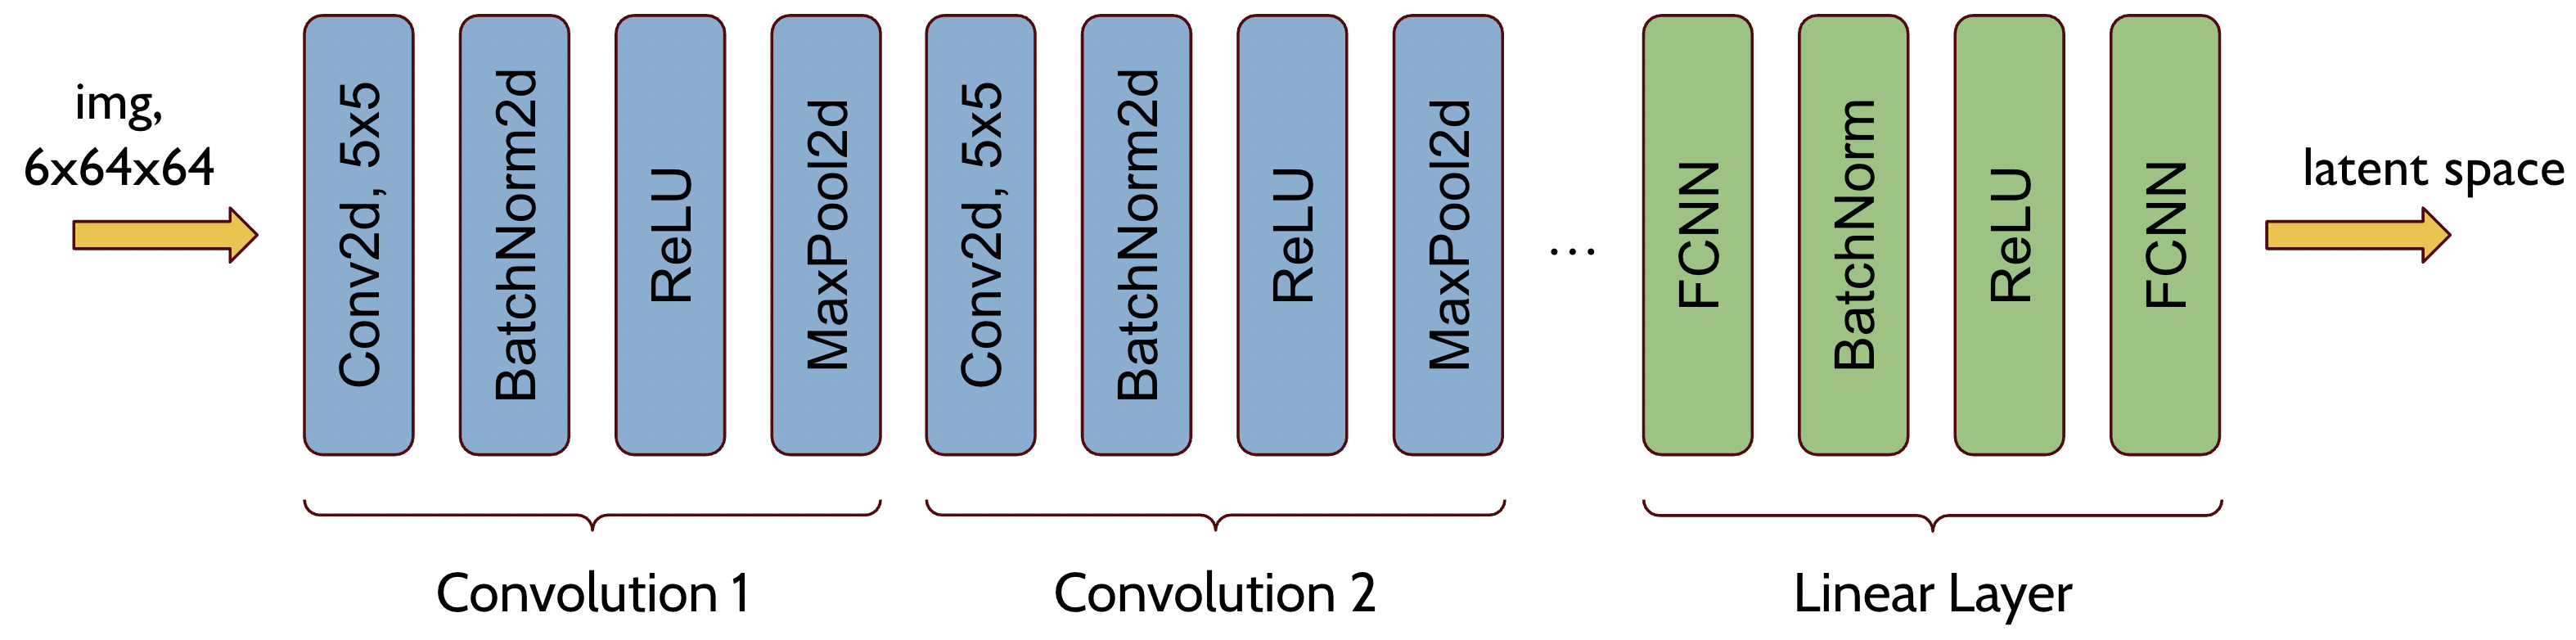
\includegraphics[width=\linewidth]{imgs/conv_diagram.png}
	\caption{Diagram for mapping from image space to GP latent space.}
	\label{fig:conv_diagram}
\end{figure}

Given the latent space feature points $z_t$, we then perform a GP regression
task over $(z_t,a_t)$ using GPyTorch \cite{GPyTorch}. The predicted probability
distribution of action over latent space from the GP model is then passed into a
Gaussian likelihood function, and the predicted novice action $a_\text{nov}$ is
defined as the mean of the likelihood.

\subsection{Uncertainty Estimation}
Similar to EnsembleDAgger \cite{ensemble-dagger}, we use the uncertainty
measurements from GP as a criterion for choosing the novice action over the
expert action in the decision rule. The uncertainty measurements from GP is
defined as the standard deviation of the likelihood.

\begin{figure}[htbp!]
	\centering
	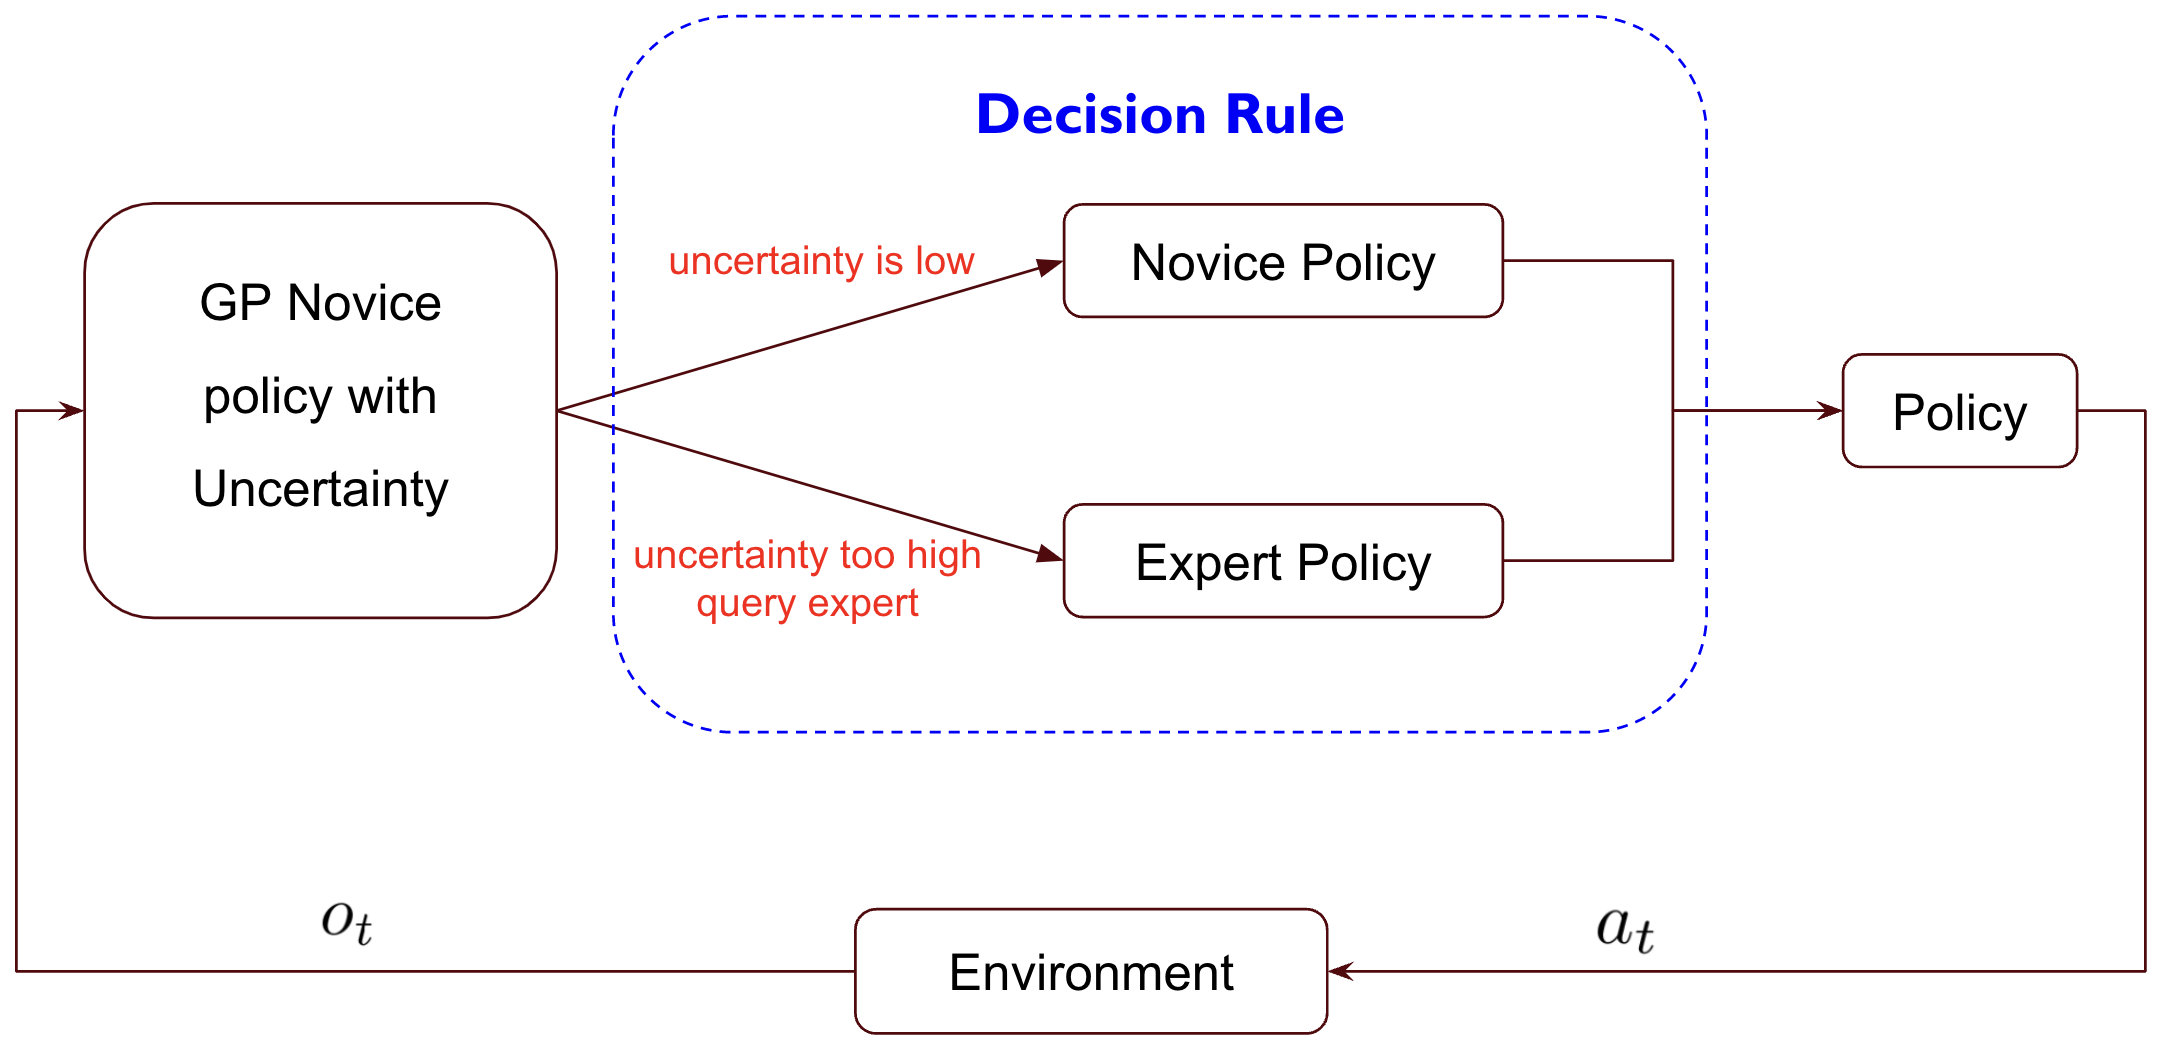
\includegraphics[width=\linewidth]{imgs/dev_dagger_diagram.png}
	\caption{Illustration of workflow for DevDAgger.}
	\label{fig:devdagger_diagram}
\end{figure}

As shown in Figure \ref{fig:devdagger_diagram}, the decision rule for DevDAgger
is that expert action $a_\text{exp}$ are only executed and queried for the given
$o_t$ whenever the novice is highly uncertain of its own action $a_\text{nov}$.
Specifically, we set an expert querying threshold for the GP output uncertainty
measurement that
\begin{equation}
	\text{Uncertainty upper bound}=\alpha \times \sqrt{\text{covar\_module.outputscale}+\text{likelihood.noise}}
\end{equation}
where $\alpha$ is a tunable hyperparameter. Whenever $a_\text{nov}$ comes with
an uncertainty higher than this upper bound, DevDAgger would query the expert
and aggregate $a_\text{exp}$ to the dataset.

Since GP is accurate in uncertainty measurements, the use of GP in regressing
latent space $\mathcal{Z}$ to action space $\mathcal{A}$ provides an accurate
estimation of novice's confidence of its own action and thus saves a lot of
expert queries than other variants of DAgger \cite{ensemble-dagger}.

\section{Experimental Results}
Our experiments focus on imitation learning with Gaussian Processes, the
potential of using Deep Kernel Learning (CNN + GP) to estimate uncertainties
from images, and eventually DevDAgger. In this section, we present experimental
validation for the following claims:
\begin{enumerate}
	\item Assuming access to the ground truth states of agents
	      \begin{enumerate}
		      \item Gaussian Processes perform well in terms of action regression
		            and uncertainty estimation.
		      \item The GP-novice policy’s output variance is a good measure of
		            dissimilarity between the query state and states in the training
		            dataset.
		      \item By purely relying on the GP's output uncertainties in the
		            DevDAgger framework, the novice policy is able to achieve better
		            performance due to high exploration coverage, despite making
		            fewer queries to the expert policy.
	      \end{enumerate}

	\item When only visual observations are given
	      \begin{enumerate}
		      \item The GP-novice policy is able to learn with significantly more
		            demonstrations.
		      \item The uncertainty estimation is highly inaccurate since the
		            learned latent space is not well structured.
		      \item Due to the above reason, DevDAgger is not able to improve query
		            efficiency when only visual observations are given.
	      \end{enumerate}
\end{enumerate}

To justify the above claims, we test our proposed approaches on a simple
cart-pole system as illustrated in Fig \ref{fig:cart-pole}. The objective of
this task is to balance the inverted pendulum by moving the cart horizontally.
The ground truth state of this cart-pole system consists of 4 dimensions $x,
	\Dot{x}, \theta, \Dot{\theta}$, where $x$ is the horizontal position of the
cart, $\theta$ is the angle of the inverted pendulum, and $\Dot{x}$ and
$\Dot{\theta}$ represent the positional velocity and angular velocity
respectively. To learn from demonstrations, we make use of a PID controller as
the expert policy. Note that this PID controller only considers $\theta$ and
$\Dot{\theta}$ and is invariant to $x$ and $\Dot{x}$.

\begin{figure}[ht]
	\centering
	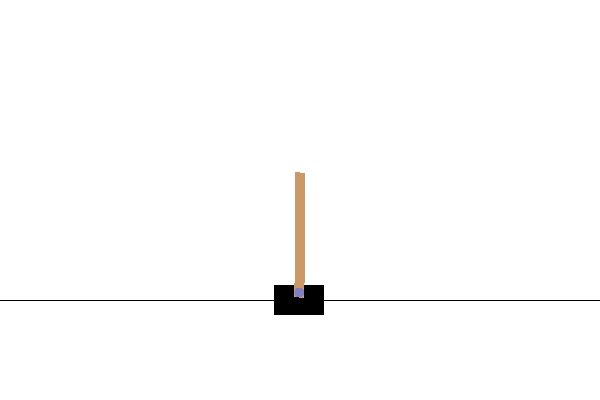
\includegraphics[width=0.5\linewidth]{imgs/random_rollout3.jpg}
	\caption{An example of the visual observation of the cart-pole system.}
	\label{fig:cart-pole}
\end{figure}

\subsection{Imitation Learning \& Uncertainty Estimation with Gaussian Processes}
\subsubsection{State-based Imitation Learning}
When the ground truth states of the cart-pole system are accessible, we use a GP
to directly regress the function mapping from states to actions based on the
demonstration dataset collected by the expert controller. One of the key
benefits of using GP is the learning efficiency, and this is supported by the
quantitative results shown in Table \ref{tab:comparison}. The state-based GP
controller is able to learn from very few examples (Fig
\ref{fig:state-il}:Left), and achieves high accuracies in the state space
covered by the training dataset, in the meantime generalizes reasonably well to
unseen states (Fig \ref{fig:state-il}:Right).

Furthermore, GP is able to model the epistemic uncertainty (Fig
\ref{fig:state-il}:Middle), in which unseen states generally correspond to high
uncertainties.

\begin{figure}[ht]
	\centering
	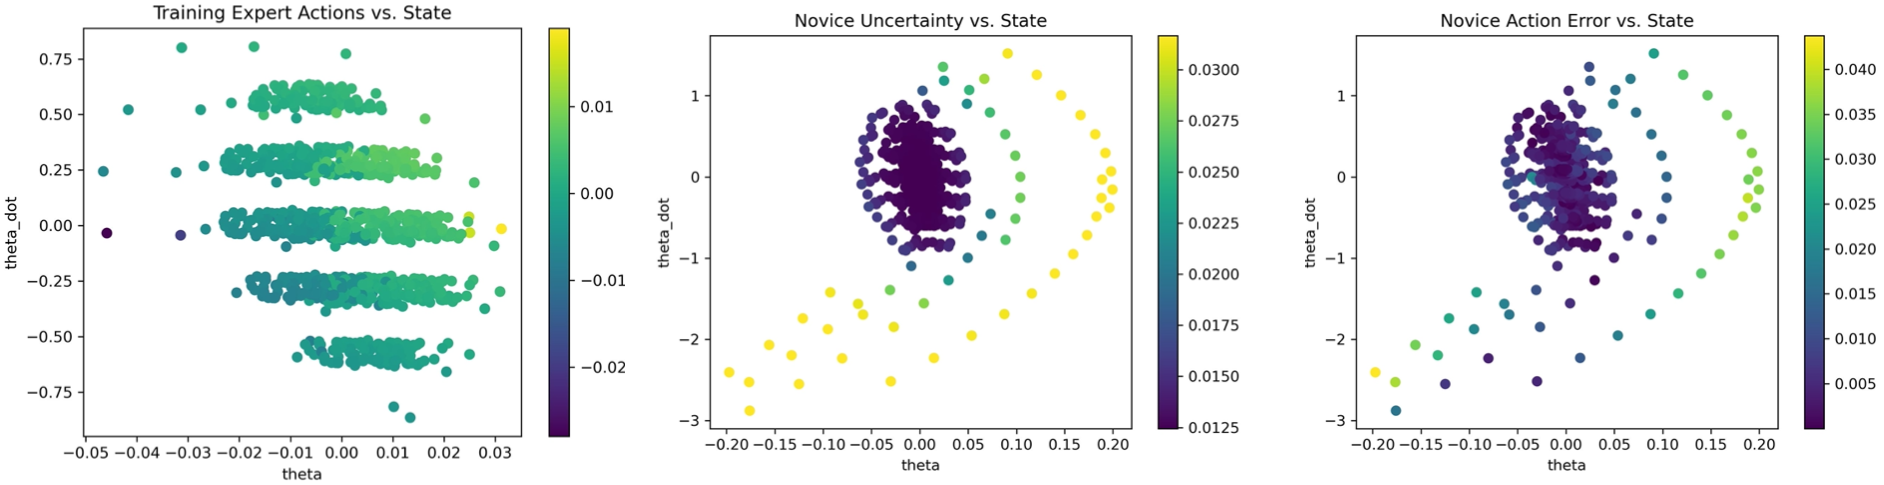
\includegraphics[width=\linewidth]{imgs/state-il.png}
	\caption{State-based imitation learning with GP. Left: visualization of the training demonstration dataset distribution, color represents the expert policy control output (target); Middle: uncertainty estimation from GP on a testing dataset, color represents uncertainty; Right: novice policy control error, color represents the absolute difference between the expert policy action and the novice policy action for a given state.}
	\label{fig:state-il}
\end{figure}

\subsubsection{Visual Imitation Learning} \label{vis-il} To explore the
possibilities of using non-parametric models like GP for high dimensional
inputs, we experiment Deep Kernel Learning with a simple imitation learning
task. Note that doing visuomotor control is an inherently difficult task in the
sense that the model must learn to extract visual features. We stack two
adjacent images together to feed in velocity information. Compared with
state-based IL, visual IL  achieves worse performance despite requiring more
training data (Table \ref{tab:comparison}).

We further visualize the uncertainty estimation on the testing dataset in Fig
\ref{fig:visual-il}:Middle, and discover that the epistemic uncertainties are
not correctly modeled by Deep Kernel Learning, as two observations correspond to
very different uncertainties even though their ground truth states are extremely
close.

\begin{figure}[ht]
	\centering
	% 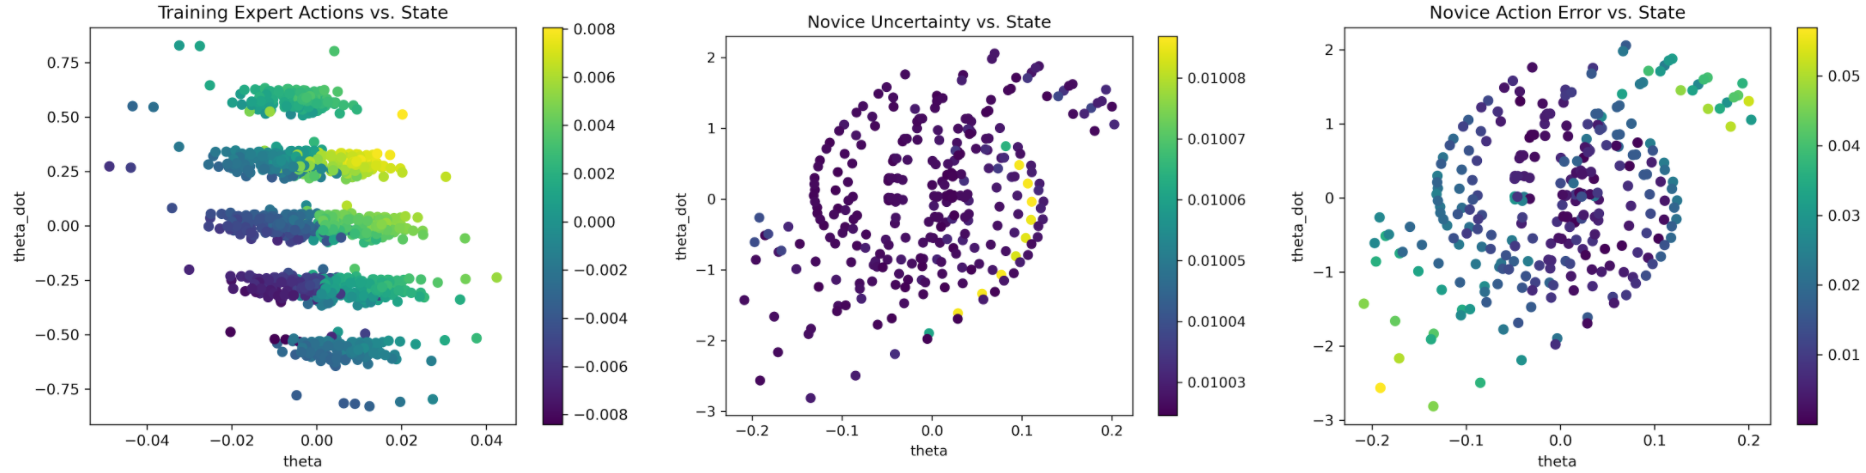
\includegraphics[width=\linewidth]{imgs/visual-il.png}
	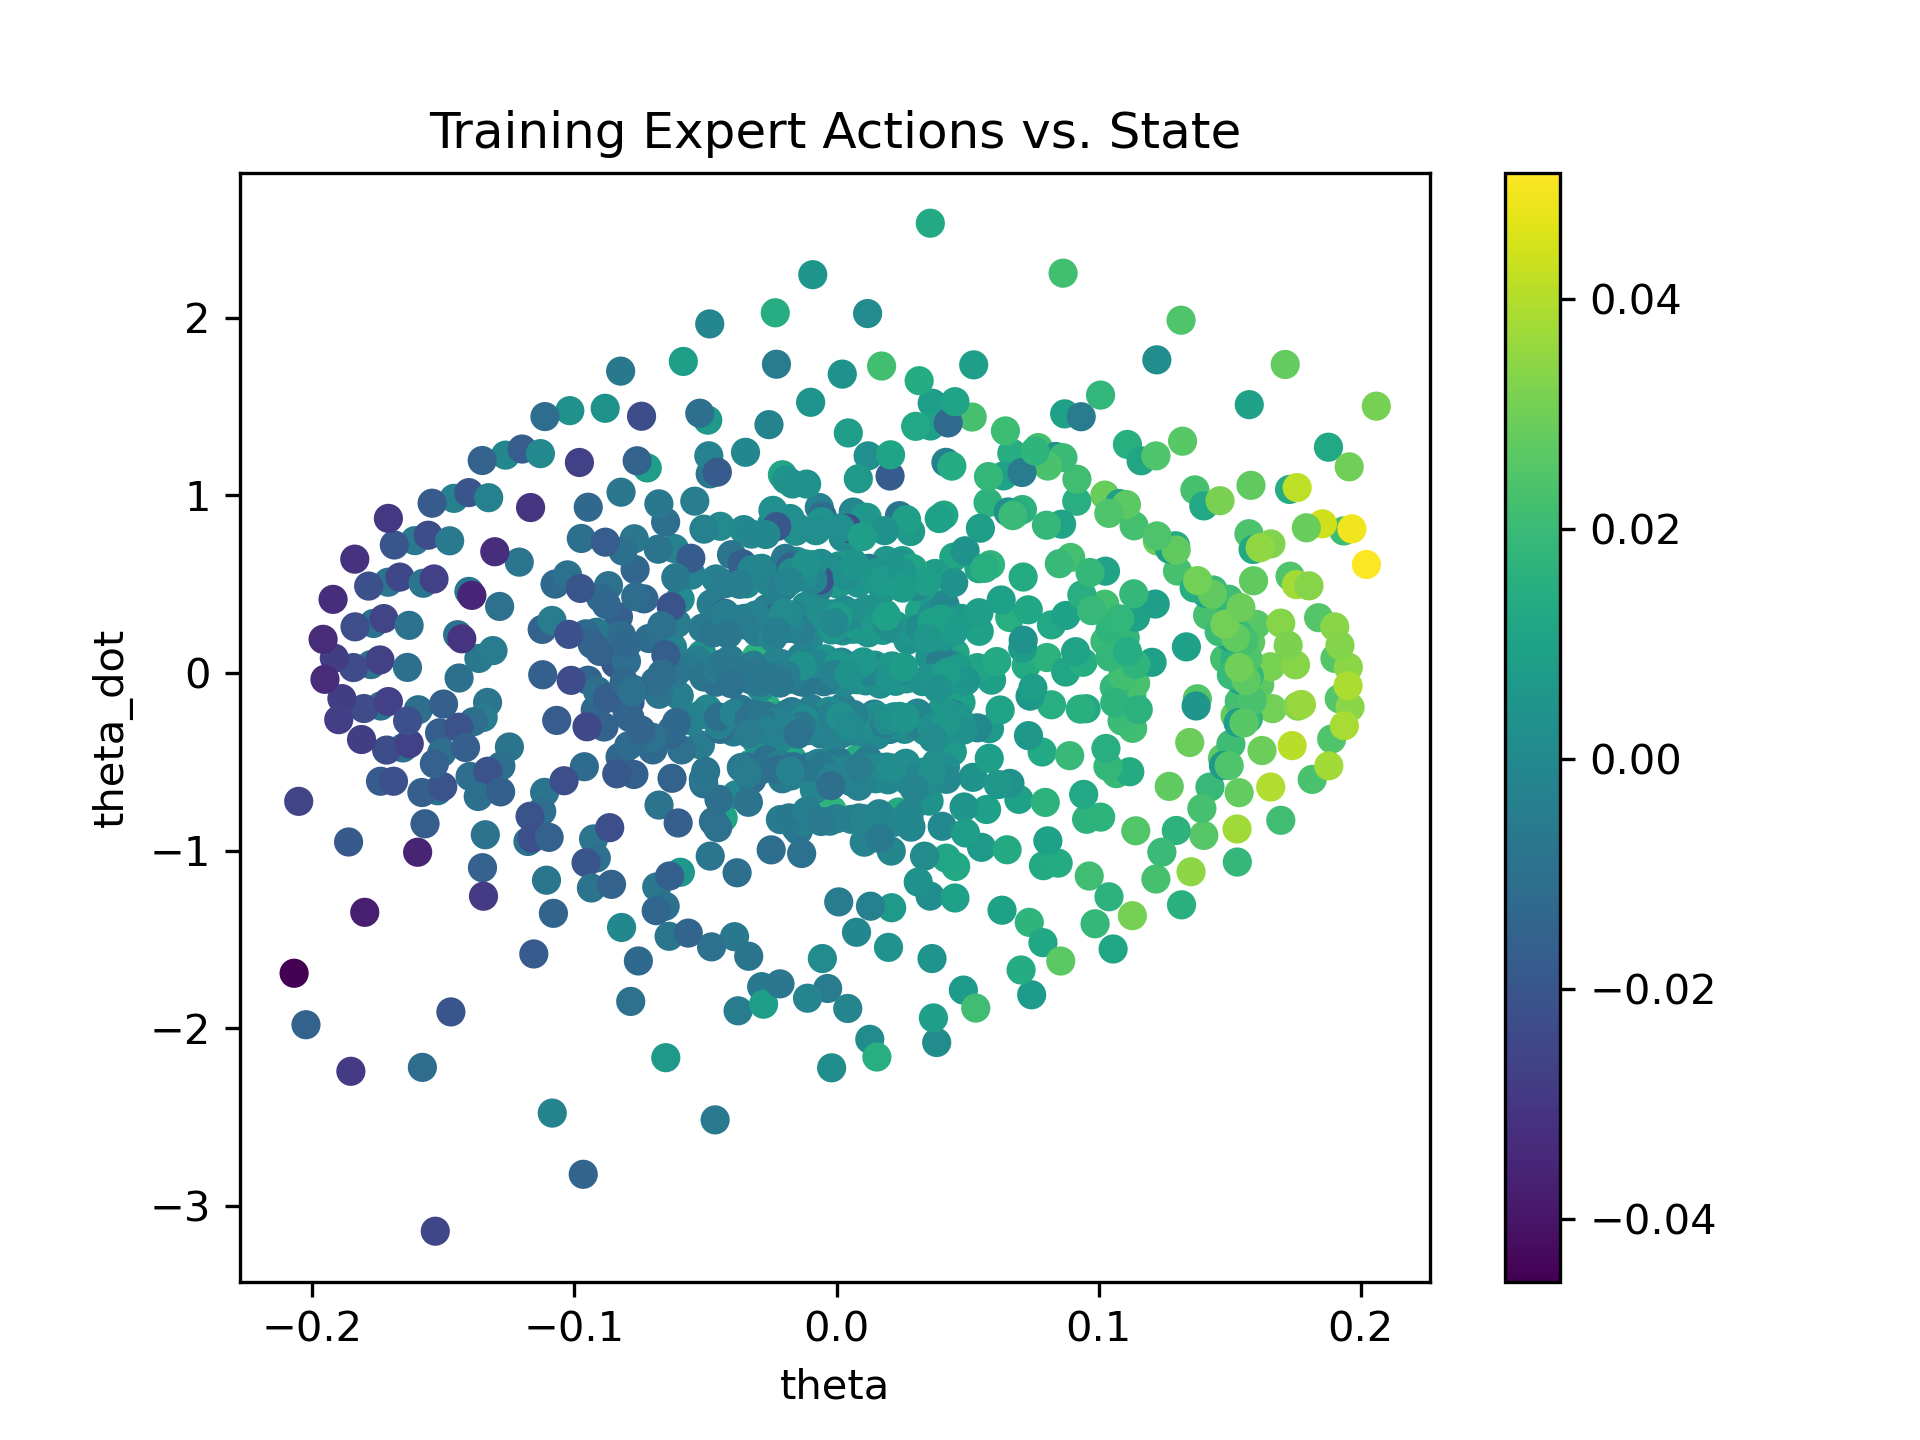
\includegraphics[width=0.32\linewidth]{imgs/expert_data_0.png}
	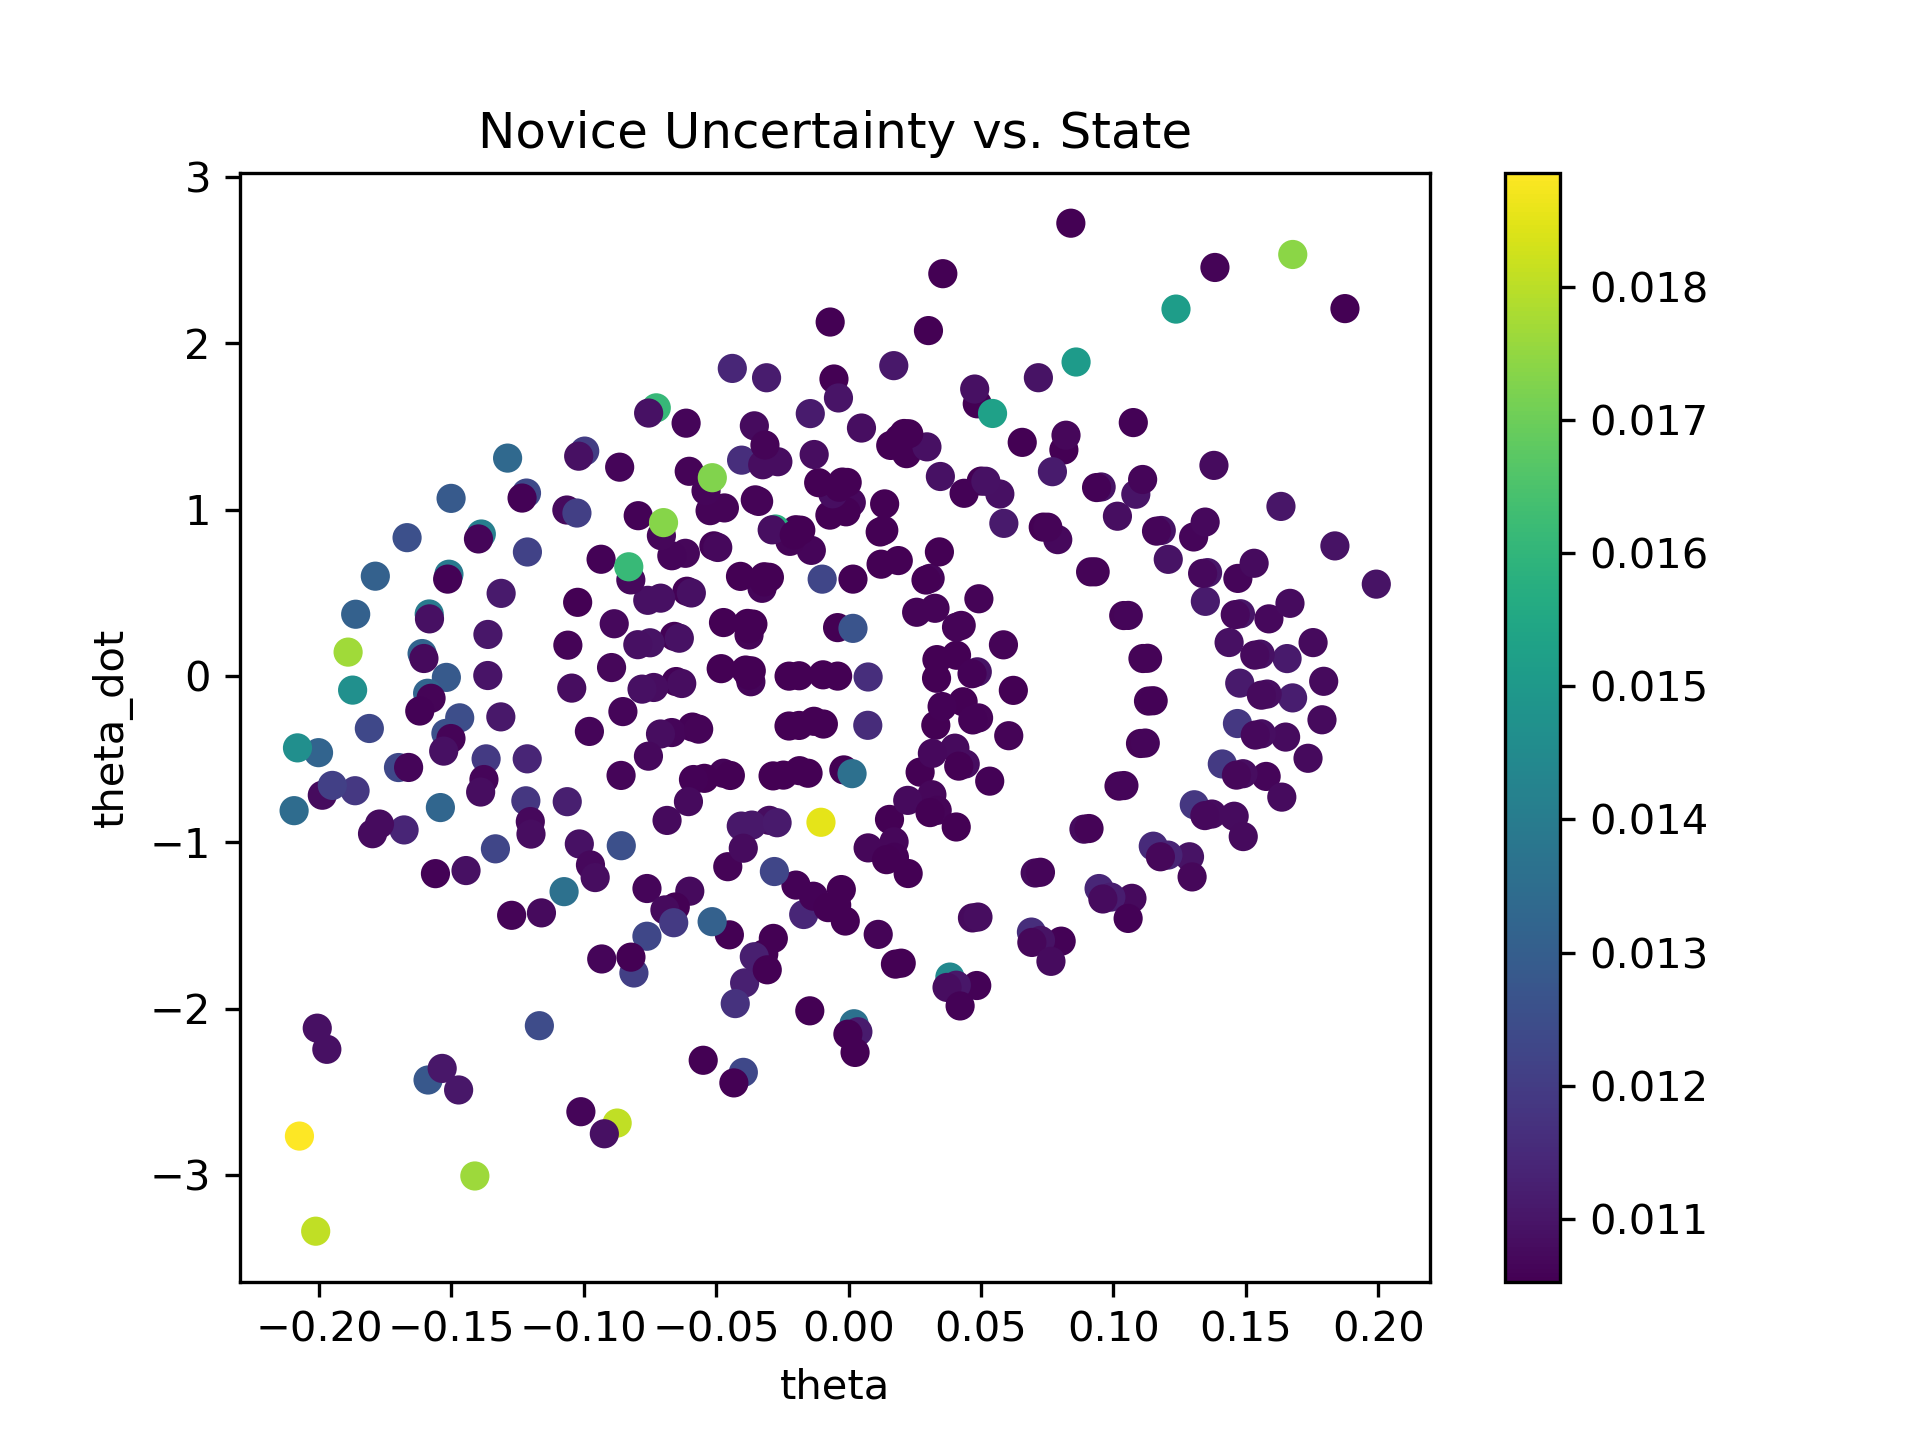
\includegraphics[width=0.32\linewidth]{imgs/novice_uncertainty_0.png}
	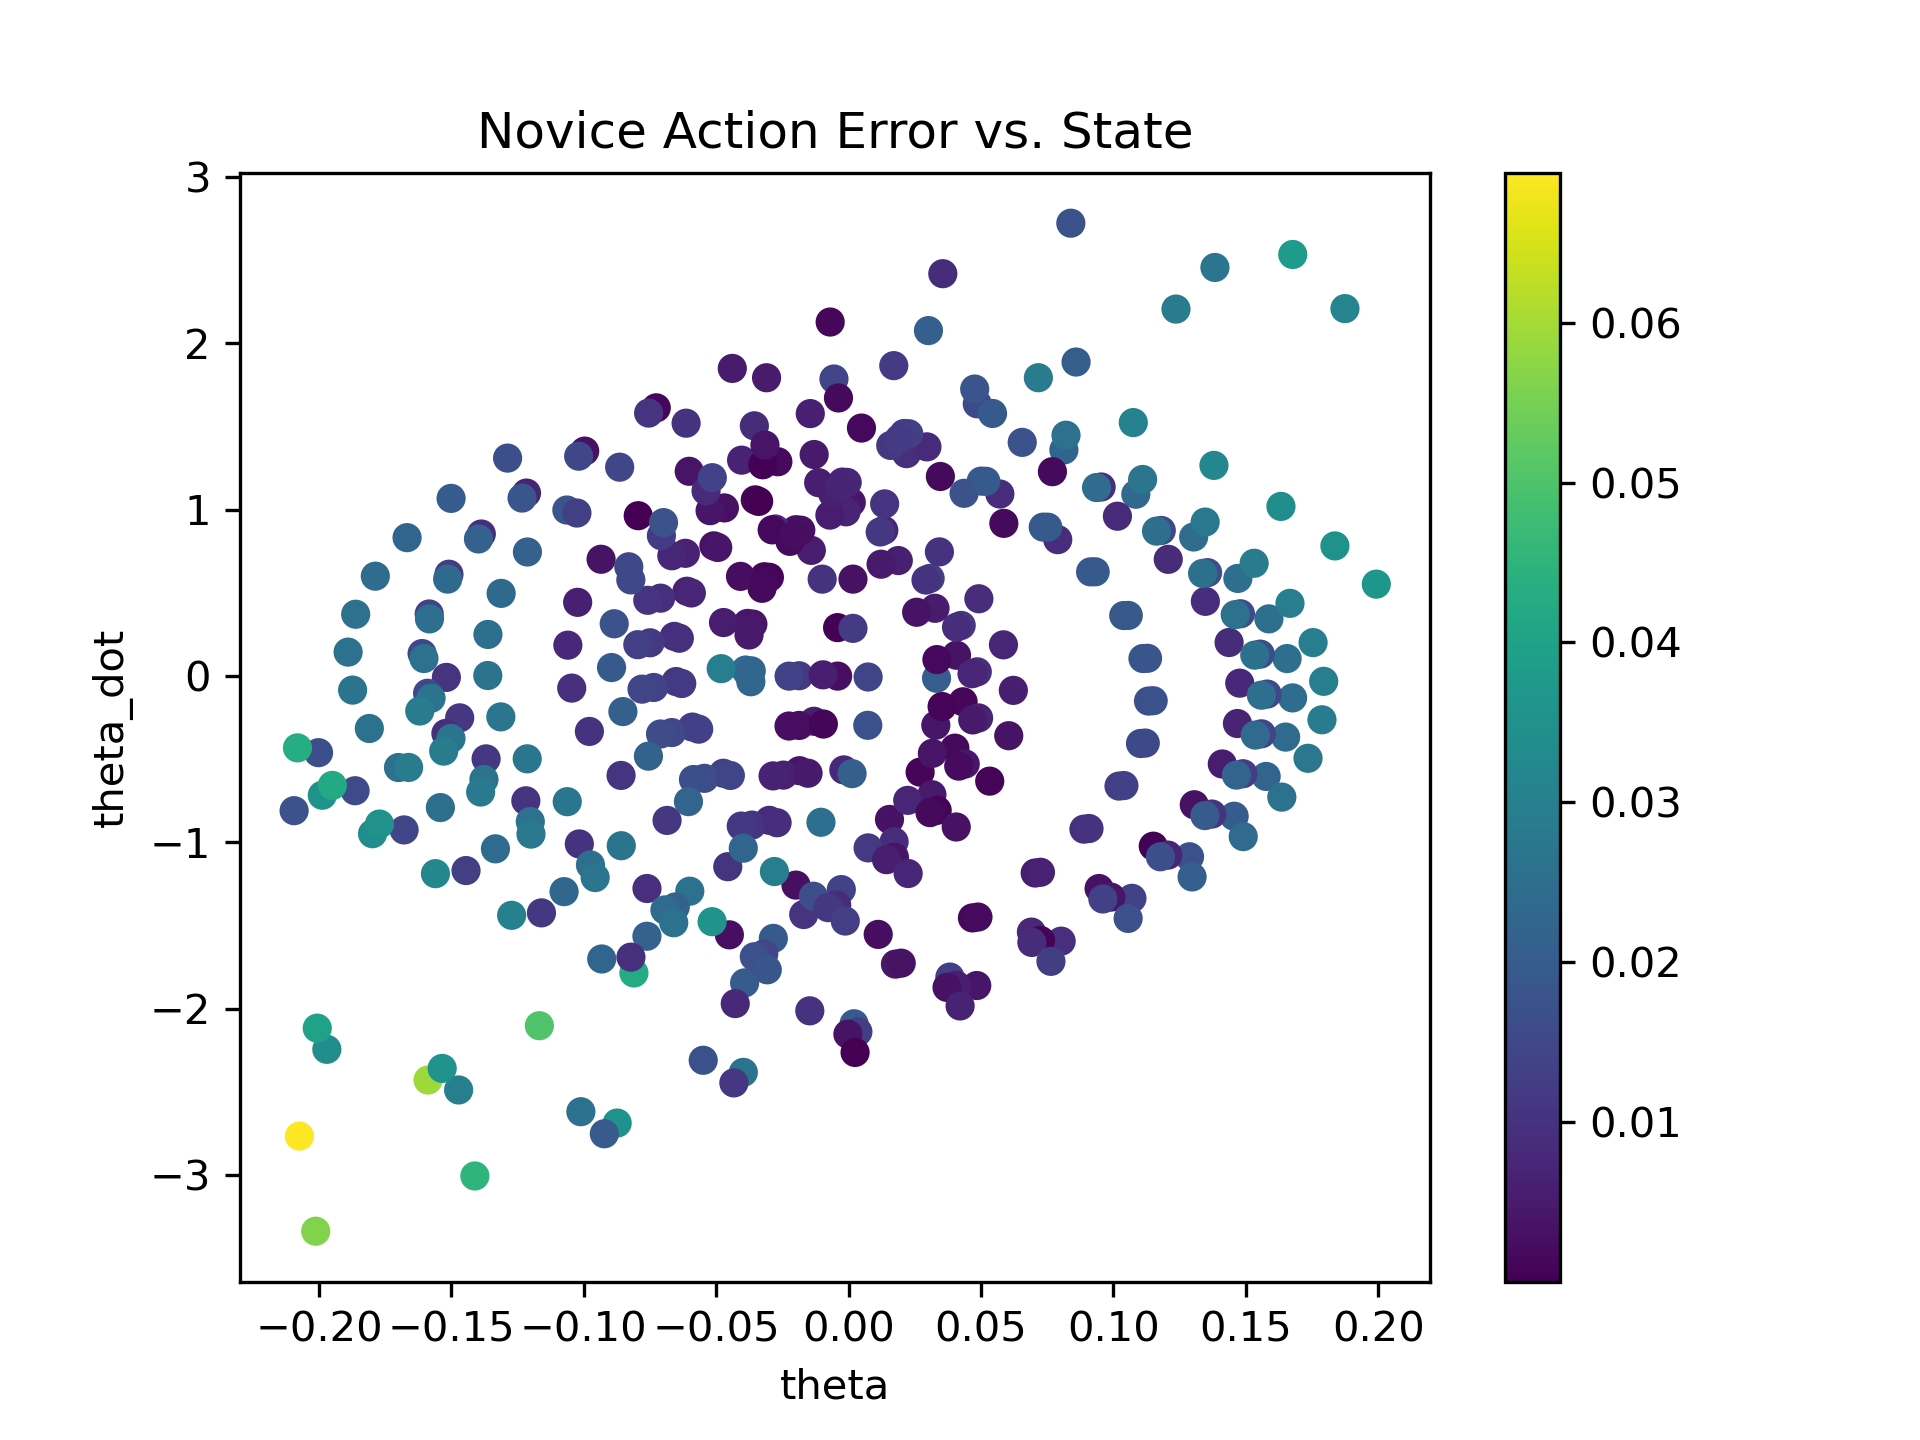
\includegraphics[width=0.32\linewidth]{imgs/novice_error_0.png}
	\caption{Visual imitation learning with GP.}
	\label{fig:visual-il}
\end{figure}

To investigate this issue of uncertainty estimation, following the visualization
protocol presented in prior work ``Embed to control'' \cite{watter2015embed}, we
set the CNN output latent space to be 2-dimensional, and visualize the mapping
between the state space and the latent space as shown in Fig \ref{fig:latent}.
Ideally the CNN would be forced to extract the true state information from
visual observations. However, the Deep Kernel Learning model fails to discover
the underlying structure of the state space. Our hypothesis for this phenomenon
is that the image distance does not reflect the actual state distance, thus,
without constraints, the model naturally has no clue to learn a structured
latent space.

\begin{figure}[ht]
	\centering
	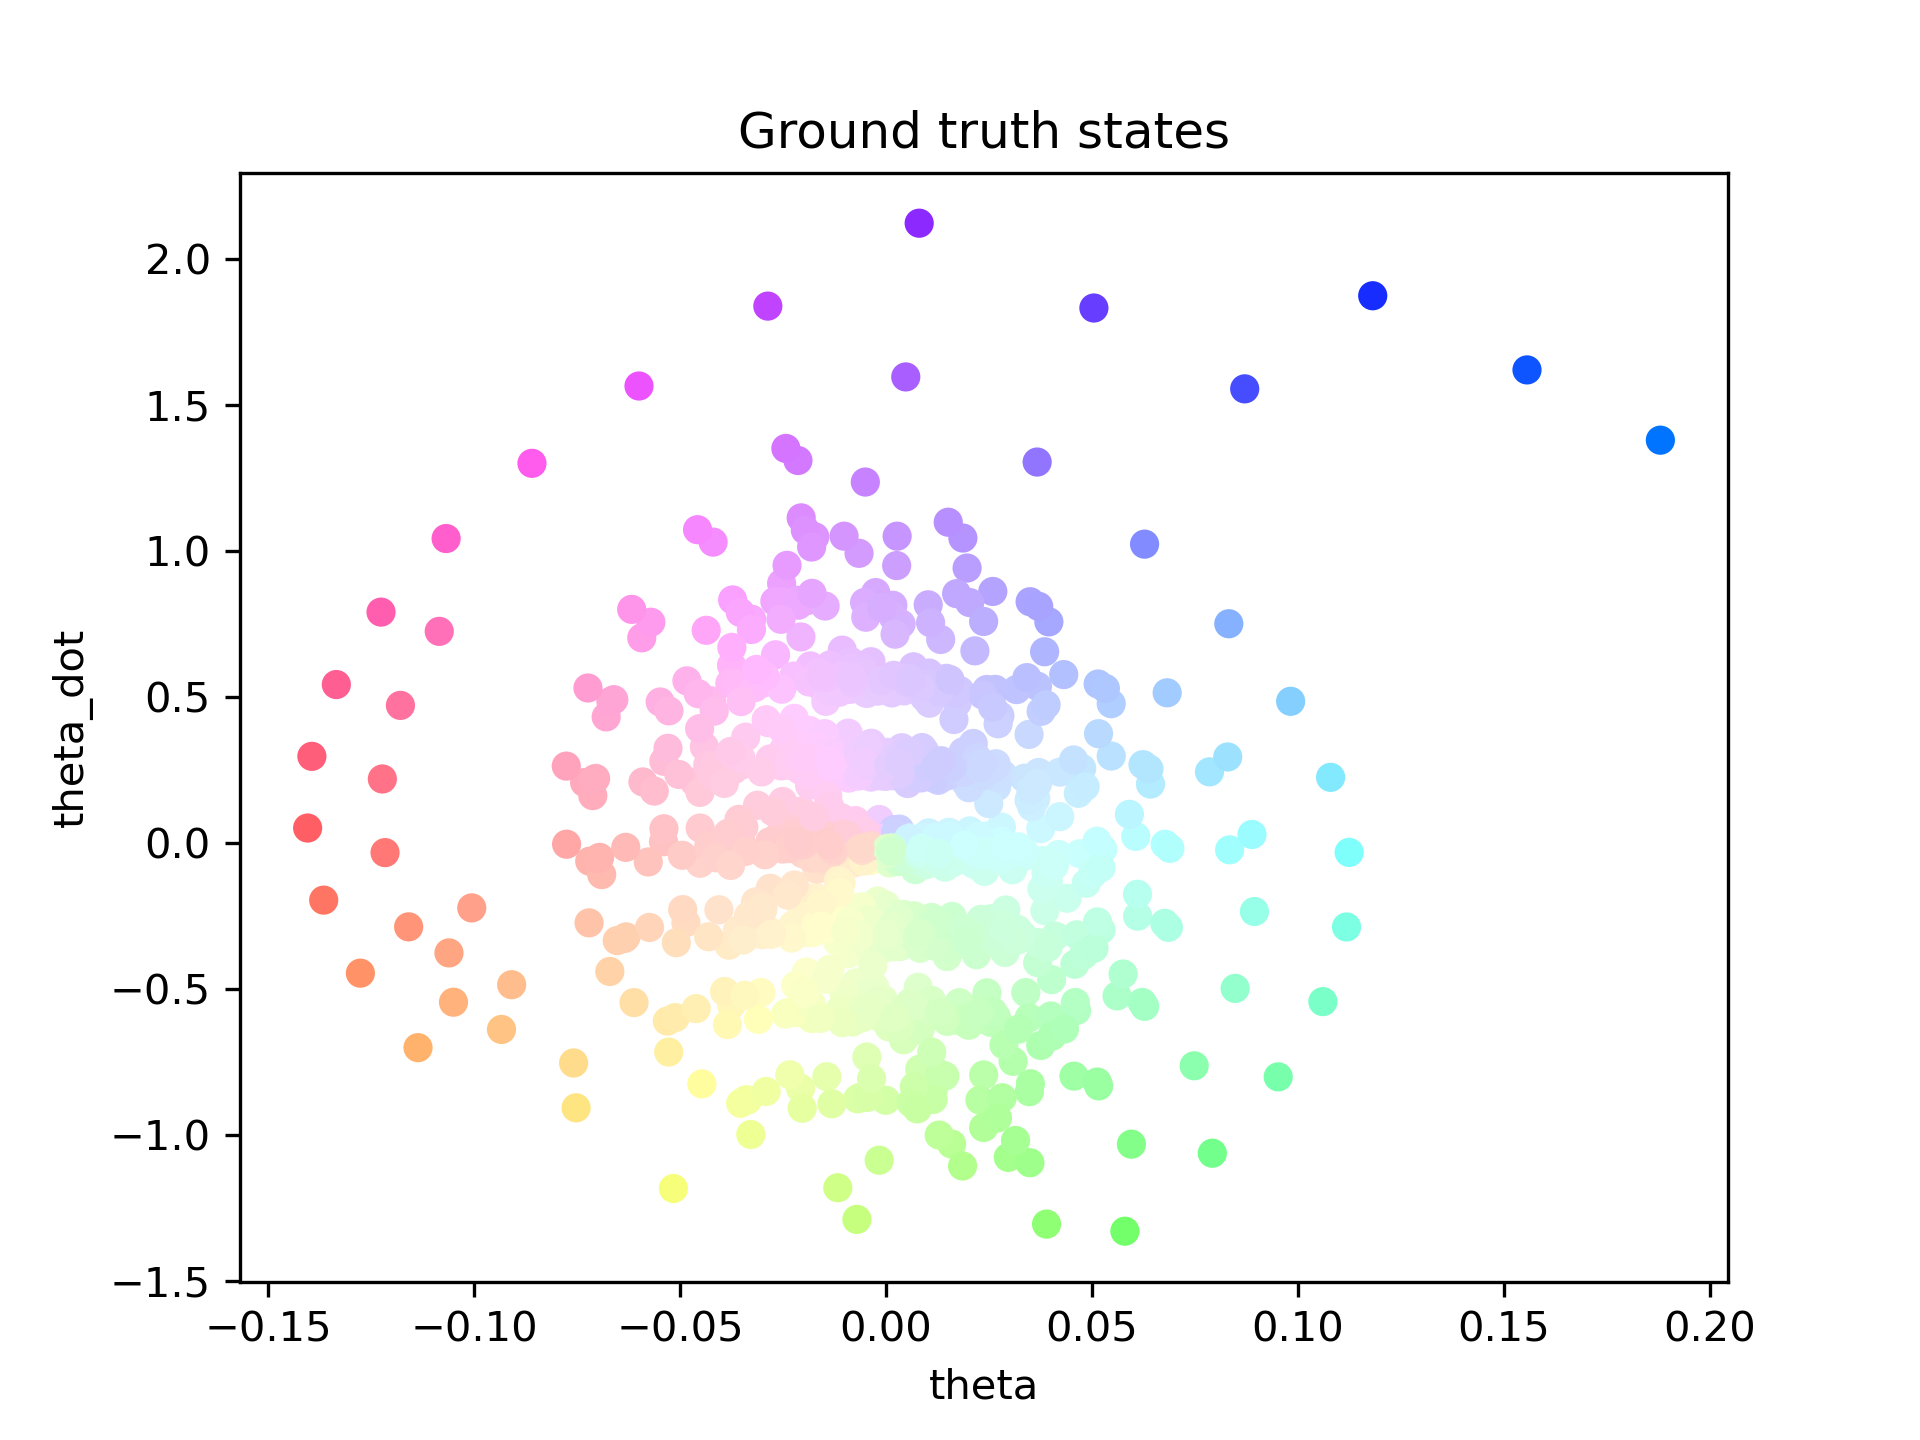
\includegraphics[width=0.4\linewidth]{imgs/latentVis_gt_states_0.png}
	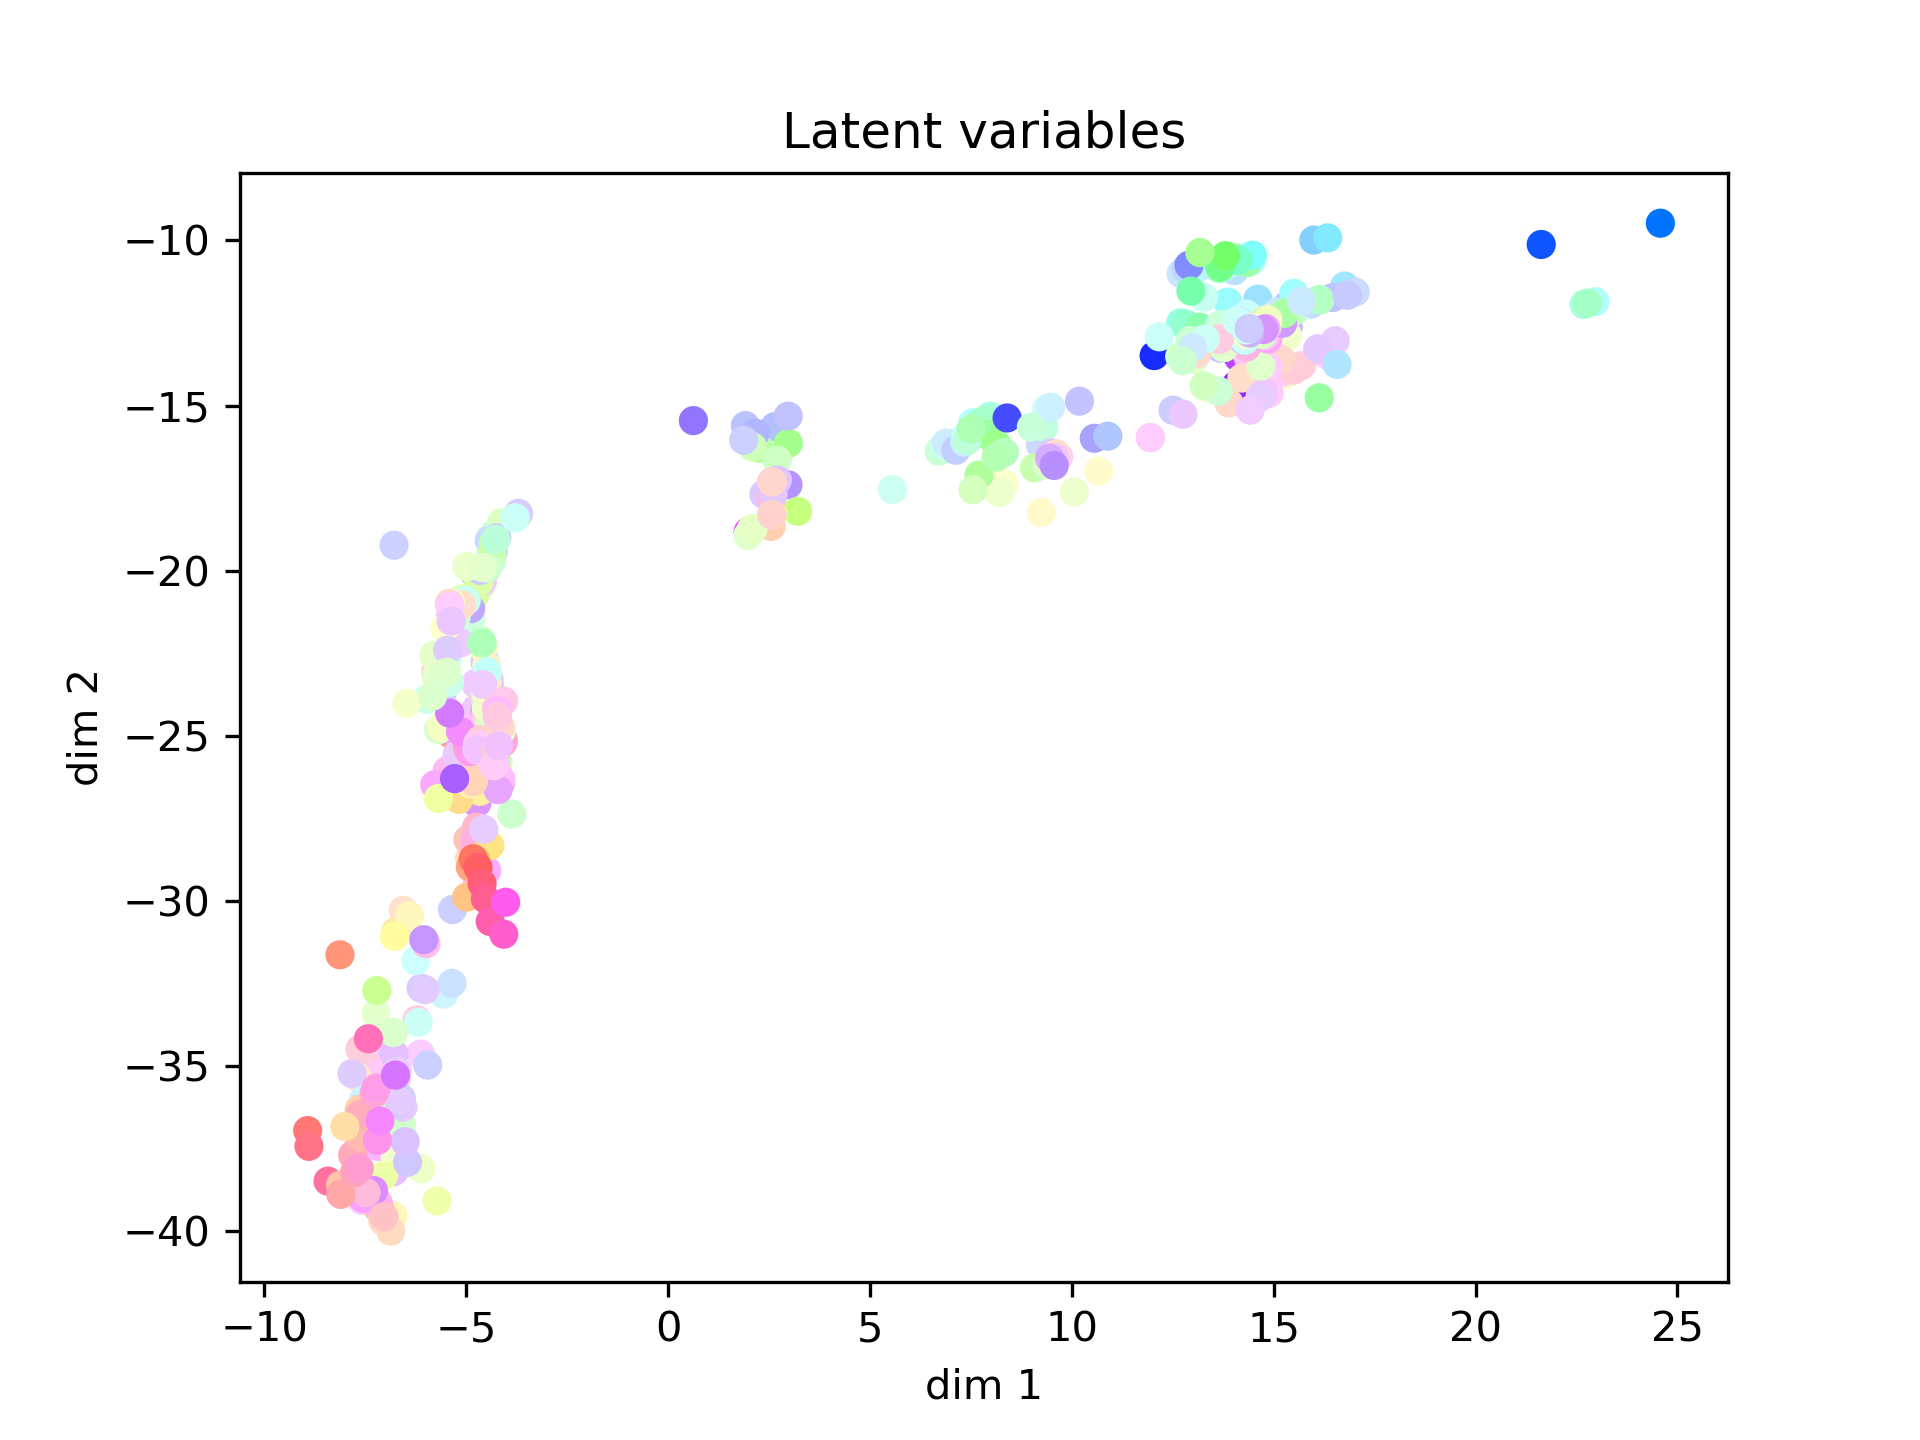
\includegraphics[width=0.4\linewidth]{imgs/latentVis_latents_0.png}
	\caption{Visualization of the latent space learned by the CNN. Left: ground truth states; Right: corresponding learned latent representations. Points in the true state space and the latent space are associated by color.}
	\label{fig:latent}
\end{figure}

\begin{table}[ht]
	\centering
	\begin{tabular}{|l|c|c|}
		\hline
		                                         & Avg Balanced Duration $\uparrow$
		                                         & Expert Query Count $\downarrow$
		\\
		\hline
		State-based IL                           & 67.1                             & 200.0
		\\
		\hline
		State-based DevDAgger                    & \textbf{74.08}                   & \textbf{178.4}
		\\
		\hhline{|=|=|=|}
		Visual IL                                & \textbf{45.87}                   & 1000.0
		\\
		\hline
		Visual Vanilla DAgger ($\gamma = 0.995$) & 35.6                             & 1000.0
		\\
		\hline
		Visual Vanilla DAgger ($\gamma = 0.999$) & \textbf{45.3}                    & 1000.0
		\\
		\hline
		Visual DevDAgger                         & \textbf{43.15}                   & \textbf{613.3}
		\\
		\hline
	\end{tabular}
	\caption{Quantitative comparison between different approaches in terms of both the average number of time steps during which the inverted pendulum is balanced, and the number of queries made for the expert policy. Each approach is at least tested for 50 trials.}
	\label{tab:comparison}
\end{table}

\subsection{DevDAgger: Uncertainty-based Decision Rule for DAgger}
We further experiment with incorporating uncertainty estimation into online
imitation learning algorithm DAgger.

\subsubsection{State-base DevDAgger}
The uncertainty-based decision rule is set as followings: if the predicted
uncertainty is larger than $\alpha \sigma_{prior}$ where $\alpha=0.7$, query the
expert policy for what action $a$ to take, and aggregate this new state-action
pair $(s, a)$ to the current dataset; otherwise, rollout the current novice
policy.

With each newly aggregated state-action pair, ideally we would train the GP
model again, however, an exact GP model is trained every $30$ data collection
steps with the aim to improve runtime efficiency.

The quantitative comparison between the state-based IL and the state-based
DevDAgger in Table \ref{tab:comparison} shows that the proposed
uncertainty-aware decision rule is able to learn a better policy with fewer
expert queries in an online fashion given the ground truth states.

\subsubsection{Visual DevDAgger}
We use the same uncertainty threshold $\alpha$, and experimented with different
latent space dimensions $2, 4, 8, 16$. As discussed in section \ref{vis-il}, the
uncertainty estimation of the Deep Kernel Learning model is very problematic due
to the unstructured learned latent space. This phenomenon causes the
unreasonable behavior of the uncertainty-aware decision rule and fails to
improve the performance compared with visual imitation learning (Table
\ref{tab:comparison}).

\section{Future Work}
To resolve the issue with the uncertainty estimation of visual GP imitation
learning, a structured latent space has to be enforced by adding constraints to
the model. A very simple solution would be to train a regression model that
predicts the ground truth states from images. We can also use contrastive
learning to enforce the structure in the learned latent space. However, both of
these two methods rely on supervision, i.e. providing ground truth states as
labels for each image.

Without ground truth states as supervision, proposed by \cite{watter2015embed},
we could train a dynamics model in the latent space and force the dynamical
model to be linear. As an extension to \cite{watter2015embed}, a more recent
work \cite{levine2019prediction} achieves better results in terms of the latent
space structure.

\section{Conclusion}
We propose DevDAgger, a data-efficient vision-based algorithm for online
imitation learning. Compared with other variants of DAgger, DevDAgger takes the
advantage of Gaussian Processes (GP) and GPyTorch \cite{GPyTorch} in robot state
space --- action space regression tasks for accurate uncertainty measurements.
With accurate uncertainty measurements, expert queries can be reduced, which
makes the DAgger process data-efficient. CNN is also put in use in order to
achieve vision-based robot planning and control, which is of high significance
in the ongoing imitation learning research areas.

In our experiments, we tested our DevDAgger algorithm on a simple cart-pole
problem and demonstrated that in state-based imitation learning, GP is able to
model the epistemic uncertainty well. State-based DevDAgger is also able to
outperform Vanilla DAgger both in performance and in expert queries. However,
more investigations are needed in visual imitation learning and visual DAgger.

Future work includes enforcing a structured latent space by adding constraints
to the model, and training a dynamics model in the latent space to provide more
robot-specific information to the DAgger problem.

\clearpage
{
	\bibliographystyle{IEEEtranN}
	\bibliography{egbib}
}

\end{document}